\part*{تنظیمات بیشتر}
\chapter{تنظیمات MySQl و PHP}

در قسمت قبل به نحوه اتصال به سندباکس از طریق اس‌اس‌اچ پرداختیم؛ همچنین آموزش تنطیم آپاچی که یکی از موارد مهم در ایجاد یک سرور است را نیز بررسی کردیم. آپاچی یک ابزار کارساز وب است که در اکثر کارسازهای وب امروزی بهره‌مند از گنو/لینوکس و بی‌اس‌دی مورد استفاده قرار می‌گیرد. مجوز انتشار این ابزار مجوز انتشار آپاچی است که توسط بنیاد آپاچی معرفی شده است.

در این قسمت، نحوه تنظیم پی‌اچ‌پی و مای‌اس‌کیوال و مای‌اس‌کیوال ورک‌برنچ 
\lr{ MySQL Workbrench }
 را  نیز بررسی خواهیم کرد. پی‌اچ‌پی یک زبان برنامه‌نویسی اسکریپتی است که برای اجرا نیاز به تفسیر دارد. کدهای نوشته شده در زبان پی‌اچ‌پی بعد از تفسیر به صورت اچ‌تی‌ام‌ال در آمده و به سمت کاربر ارسال خواهند شد. با این حال برخی تنظیمات و سفارشی‌سازی در استفاده و عملکرد این زبان برنامه‌نویسی و تفسیر کدها تاثیر زیادی دارند؛ همانطور که در قسمت اول مقاله  به تفصیل بیان کردیم؛ مای‌اس‌کیوال نیز یک مدیر بانک اطلاعاتی است که برای مدیریت و دسترسی به بانکهای اطلاعاتی به کار می‌رود.  همانطور که در قسمت اول گفته شد؛ این ابزار یک ابزار متن‌باز است که در دو نسخه متن‌باز و تجاری عرضه شده‌است. پس با ما همراه باشید تا با استفاده از تنظیمات مورد نیاز برای این ابزار، یک سرور مناسب برای توسعه نرم‌افزارهای وب به صورت سند‌باکس ایجاد کنیم.

اگر فصل قبل این آموزش یعنی قسمت دوم را مطالعه کرده‌باشید؛ ابزار کارساز  آپاچی را در اوبونتو  سرور سندباکس به طور کامل تنظیم کردیم؛ به شکلی که بعد از انجام مراحل بالا، حی قادر هستیم؛ صفحه ایجاد شده توسط پی‌اچ‌پی را نیز اجرا کنیم. با وجود این موارد ذکر شده؛  اگر می‌خواهید پی‌اچ‌پی قابلیت‌های بیشتری داشته باشد و بتوانید دستورات پیشرفته و بیشتری را در این زبان اجرا کنید؛ با این قسمت از آموزش نحوه نصب اوبونتو در سندباکس همراه باشید. در این قسمت به نحوه فعال کردن نمایش پیغام خطا و رفع ایراد از کدهای پی‌اچ‌پی نوشته شده و همچنین دسترسی به مای‌اس‌کیوال به صورتی راحت نیز خواهیم رسید که بسیار کاربردی خواهند بود.
\section{پی‌اچ‌پی و تنظیمات مورد‌نیاز}

بر اساس تعریف ویکی‌پدیا:«پی‌اچ‌پی (به انگلیسی: 
\lr{PHP}
) یک زبان برنامه‌نویسی است که برای طراحی وب توسعه یافته‌است، اما می‌توان از آن به عنوان یک زبان عمومی نیز استفاده‌کرد. تا ژانویه سال ۲۰۱۳ میلادی پی‌اچ‌پی بر روی ۲۴۴ میلیون وب‌گاه و ۲٫۱ میلیون سرور وب نصب شده‌است. این زبان در سال ۱۹۹۵ میلادی توسط راسموس لِردورف (به انگلیسی:
 \lr{Rasmus Lerdorf}
 ) شناخته‌شده و در حال حاضر توسعه آن بر عهده گروه پی‌اچ‌پی می‌باشد. در ابتدا پی‌اچ‌پی از عبارت صفحه خانگی شخصی (به انگلیسی:
  \lr{ "Personal Home Page" }
  ) گرفته شده‌بود. اما اکنون این کلمه مخفف بازگشتی 
  \lr{ "PHP: Hypertext Preprocessor" }
  به معنی پی‌اچ‌پی: پیش‌پردازنده ابرمتن می‌باشد.

کدهای پی‌اچ‌پی توسط یک سرور وب که نرم‌افزار پی‌اچ‌پی بر روی آن نصب باشد، تفسیر می‌شوند. دستورهای این زبان می‌توانند به صورت مستقیم در درون کدهای اچ‌تی‌ام‌ال قرار بگیرند. زبان پی‌اچ‌پی از نسخهٔ ۴٫۳ به بعد قابلیت پشتیبانی از واسط خط فرمان را نیز به امکانات خود اضافه کرد. این قابلیت می‌تواند برای ایجاد نرم‌افزارهای غیر وبی و یا نرم‌افزارهایی با واسط گرافیکی کاربر مورد استفاده قرار بگیرد.

پی‌اچ‌پی یک نرم‌افزار آزاد است که تحت مجوز پی‌اچ‌پی انتشار یافته است. این مجوز به دلیل قرار دادن محدودیت بر روی استفاده از عنوان پی‌اچ‌پی، با مجوز همگانی گنو (GPL) سازگار نیست. پی‌اچ‌پی را می‌توان بر روی اکثر سرورهای وب نصب کرد. همچنین قابلیت نصب آن به صورت یک شل جداگانه بر روی تقریباً تمامی سیستم‌های عامل و پلت‌فرم‌ها (یا سکوها) وجود دارد. تمامی این استفاده‌ها رایگان است.» 

\begin{flushleft}
    (ویکی‌پدیا دانشنامه آزاد)
\end{flushleft}

اولین چیزی که در سرور بعد از تنظیم آپاچی، آن را تنظیم می‌کنیم؛ نرم‌افزار پی‌اچ‌پی است که همانطور که گفته شد مسئول تفسیر کدها و فایل‌های پویای پی‌اچ‌پی و تبدیل آنان به کدهای ایستای اچ‌تی‌ام‌ال است. فایل‌های پویا فایل‌هایی هستند که مقادیر و اطلاعات آنان به صورت پویا تغییر کرده و به صورت ثابت در سرور ذخیره نشده‌اند. یکی از مواردی که معمولا کاربران برای محیط‌های سندباکس و آزمایشی نیاز دارند؛ این است که بتوانند خطاهای رخ داده را مشاهده نمایند. یعنی اگر خطایی در کدهای آنان وجود داشت، پیغام خطا و هشداری مرتبط با خطای رخ‌داده در خروجی نمایش داده شود. به صورت پیش‌فرض در پی‌اچ‌پی خطاها نمایش داده نخواهند شد. به عنوان نمونه اگر دستورات زیر را در یک فایل پی‌اچ‌پی ذخیره کنید؛ با وجود اینکه این دستورات دارای خطای فاحش هستند؛ نیز پیغامی در خروجی مبنی بر رخ دادن خطا، نمایش داده نخواهد شد.
\newline
\begin{latin}
    
    \lstinputlisting[numbers=right,language=PHP, framexleftmargin=5mm, frame=shadowbox,rulesepcolor=\color{Blue}]{Code/error.php}
\end{latin}

کد‌های بالا را با نام 
\path{«errors.php»}
 در شاخه به اشتراک گذاشته شده بین سیستم میزبان سند‌باکس ذخیره کنید. سپس با نوشتن آدرس فایل به همراه نام سرور سندباکس، صفحه زیر برای شما نمایش داده خواهد شد. \ref{UbuntuServer-PHP}
\newline
\begin{figure}
    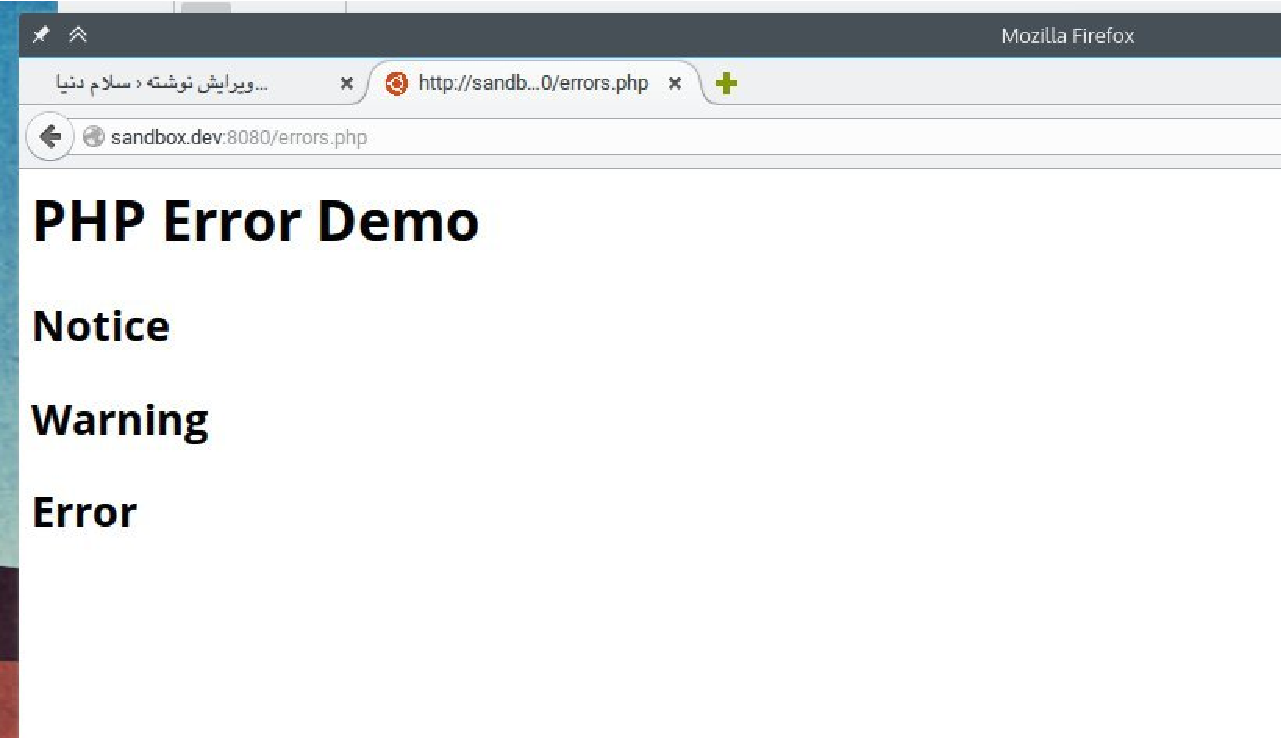
\includegraphics[width=.9\textwidth ,height=.55\textwidth]{Pic/PHP1}
    \caption{ نمایی از  نمایش خطا هنگامی که به درستی تنظیم نشده است}
    \label{UbuntuServer-PHP}
\end{figure}

همانطور که در بالا مشخص است؛ پیغام خطایی در خروجی نمایش داده نشده‌است. حال اگر می‌خواهید در صورت وجود خطایی خاص، آن خطا در خروجی نمایش داده شود باید از تنظیمات پی‌اچ‌پی، نمایش خطاها را فعال کنید. در پیغام‌های نمایش داده شده برای نکات، خطا و هشدار هیچ اطلاعاتی نمایش داده نشده است که در صورت فعال شدن امکان نمایش خطا و هشدار، صفحه بالا به شکل دیگری نمایش داده خواهد شد.  همانند آپاچی تنظیمات پی‌اچ‌پی در شاخه 
\path{«etc/»}
قرار گرفته است. برای رفتن به شاخه تنظیمات پی‌اچ‌پی و نمایش پوشه‌ها و پرونده‌های موجود در آن از دستور زیر استفاده کنید.
\newline
\begin{latin}  
    \lstinputlisting[numbers=right,language=Bash, framexleftmargin=5mm, frame=shadowbox,rulesepcolor=\color{Black}]{Code/codephp1.sh}
\end{latin}

در شاخه مذکور، سه پوشه مشاهده می‌شود که پوشه‌های اولی و دومی جهت تنظیمات و شاخه آخر نیز همانند شاخه سایت‌های در دسترس آپاچی عمل می‌کند. در این پوشه ماژول‌های در دسترس برای استفاده قرار گرفته‌اند که با دستور خاصی، می‌توان آنان را فعال نمود. برای مشاهده محتویات درون این پوشه نیز دستورات زیر را اجرا کنید.
\newline
\begin{latin}  
    \lstinputlisting[numbers=right,language=Bash, framexleftmargin=5mm, frame=shadowbox,rulesepcolor=\color{Black}]{Code/codephp2.sh}
\end{latin}
در این شاخه ماژول‌های مختلف در دسترس را مشاهده می‌کنید؛ ماژول‌هایی برای مای‌اس‌کیوال، جی‌سون و دیگر موارد مختلف که در پوشه بالا قابل دسترسی هستند. حال بیایید نگاهی به تنظیمات واقع شده در شاخه آپاچی۲ باندازیم که در کنار پوشه ماژول‌های در دسترس قرار دارد.
\newline
\begin{latin}  
    \lstinputlisting[numbers=right,language=Bash, framexleftmargin=5mm, frame=shadowbox,rulesepcolor=\color{Black}]{Code/codephp3.sh}
\end{latin}
در این شاخه نیز تنظیمات یا در شاخه «conf.d» قرار دارند که تنظیمات این شاخه پیوندی میانبر از تنظیمات شاخه ماژول‌های دسترس هستند؛ یا اینکه در داخل فایل «php.ini» درج شده‌اند. برای تنظیم مشخصات دلخواه در پی‌اچ‌پی ما یک فایل تنظیمات دلخواه را در شاخه ماژول‌های در دسترس ایجاد کرده و سپس آن را با مقادیر داده شده پر خواهیم کرد.
\newline
\begin{latin}  
    \lstinputlisting[numbers=right,language=Bash, framexleftmargin=5mm, frame=shadowbox,rulesepcolor=\color{Black}]{Code/codephp4.sh}
\end{latin}

در فایلی که در ترمینال باز شده است مقادیر زیر را وارد کنید.
\newline
\begin{latin}  
    \lstinputlisting[numbers=right,language=Bash, framexleftmargin=5mm, frame=shadowbox,rulesepcolor=\color{Black}]{Code/codephp5.sh}
\end{latin}
تنظیمات بالا یک سری تنظیمات برای پی‌اچ‌پی هستند که در آن برخی تغییرات در مقادیر پیش‌فرض پی‌اچ‌پی انجام گرفته است. بعد از ذخیره فایل بالا؛ شما خواهید توانست که با استفاده از دستور 
\path{«php5enmod»}
 تنظیمات سفارشی مورد نظر خود را فعال کنید. برای غیر فعال کردن هر یک از تنظیمات نیز از دستور 
 \lr{«php5dismod»}
  استفاده می‌شود. به عنوان نمونه برای فعال کردن تنظیم نوشته شده و سفارشی خودمان دستور زیر را وارد می‌کنیم. تنظیمات بدون پسوندشان نوشته خواهند شد.
\newline
\begin{latin}  
    \lstinputlisting[numbers=right,language=Bash, framexleftmargin=5mm, frame=shadowbox,rulesepcolor=\color{Black}]{Code/codephp6.sh}
\end{latin}
بعد از اجرای دستور بالا ما باید یک فایل لاگ برای خطاهای پی‌اچ‌پی نیز ایجاد کنیم. برای این کار از دستور تاچ «touch» که برای ساخت فایل جدید کاربرد دارد؛ استفاده کرده و فایلی را به صورت زیر ایجاد می‌کنیم.
\newline
\begin{latin}  
    \lstinputlisting[numbers=right,language=Bash, framexleftmargin=5mm, frame=shadowbox,rulesepcolor=\color{Black}]{Code/codephp7.sh}
\end{latin}

دستور تغییر مالک «chown» برای تغییر مالک یک فایل به کاربر و یا گروه خاص استفاده می‌شود. این دستور به صورت زیر اجرا کنید؛ به این خاطر که مالکیت فایل را برای آپاچی و کاربر «www-data» در نظر گرفته و بتوانیم به این پرونده توسط این کاربر دسترسی داشته باشیم. هر پوشه‌ای که برای کاربر بالا مجاز باشد توسط آپاچی نیز قابل تغییر و مشاهده است.
\newline
\begin{latin}  
    \lstinputlisting[numbers=right,language=Bash, framexleftmargin=5mm, frame=shadowbox,rulesepcolor=\color{Black}]{Code/codephp8.sh}
\end{latin}
چند ماژول دیگری هم که در اکثر مواقع توسط توسعه‌دهندگان پی‌اچ‌پی استفاده می‌شود را نیز با استفاده از دستورات زیر نصب و فعال می‌کنیم. ابتدا بسته‌های نرم‌افزاری زیر را توسط ای‌پی‌تی نصب کنید؛ تا بتوانید با استفاده از دستور فعال کردن ماژول آنان را فعال کنید. این ابزار شامل ابزار بانک اطلاعاتی بسیار سبک و پر قدرت اسکیو‌لایت و ابزار رمزنگاری ام‌کریپت می‌شود.
\newline
\begin{latin}  
    \lstinputlisting[numbers=right,language=Bash, framexleftmargin=5mm, frame=shadowbox,rulesepcolor=\color{Black}]{Code/codephp9.sh}
\end{latin}
بعد از نصب بسته‌های نرم‌افزاری بالا می‌توانید در ابتدا ماژول رمزنگاری «mcrypt» را فعال کنید. برای این کار از دستور زیر استفاده خواهیم کرد. دستور زیر برای فعال کردن ماژول‌‌‌های دلخواه دیگر نیز کاربرد خواهد داشت.
\newline
\begin{latin}  
    \lstinputlisting[numbers=right,language=Bash, framexleftmargin=5mm, frame=shadowbox,rulesepcolor=\color{Black}]{Code/codephp10.sh}
\end{latin}
مابقی ماژول‌های نصب شده مانند ماژول اسکیو‌لایت «SQLite» نیز به صورت خودکار فعال خواهد بود و نیازی به نوشتن دستوری برای فعال کردن آن وجود ندارد.  بعد از آن با اجرای مجدد آپاچی ۲؛ و اجرای مجدد فایل دارای خطا به زبان  پی‌اچ‌پی؛ خطاها به شکل پیغام‌هایی در خروجی به نمایش در خواهند آمد.
\newline
\begin{latin}  
    \lstinputlisting[numbers=right,language=Bash, framexleftmargin=5mm, frame=shadowbox,rulesepcolor=\color{Black}]{Code/codephp11.sh}
\end{latin}
بعد از اجرای دستور بالا، آپاچی ۲، راه‌اندازی مجدد خواهد شد و تنظیمات و ماژول‌های اعمالی به موارد تغییر یافته، به‌روز خواهند شد. بعد از آن اگر آدرس فایل را در سند‌باکس باز کنید؛ تصویری مشابه تصویر را مشاهده خواهید کرد.
\begin{figure}
    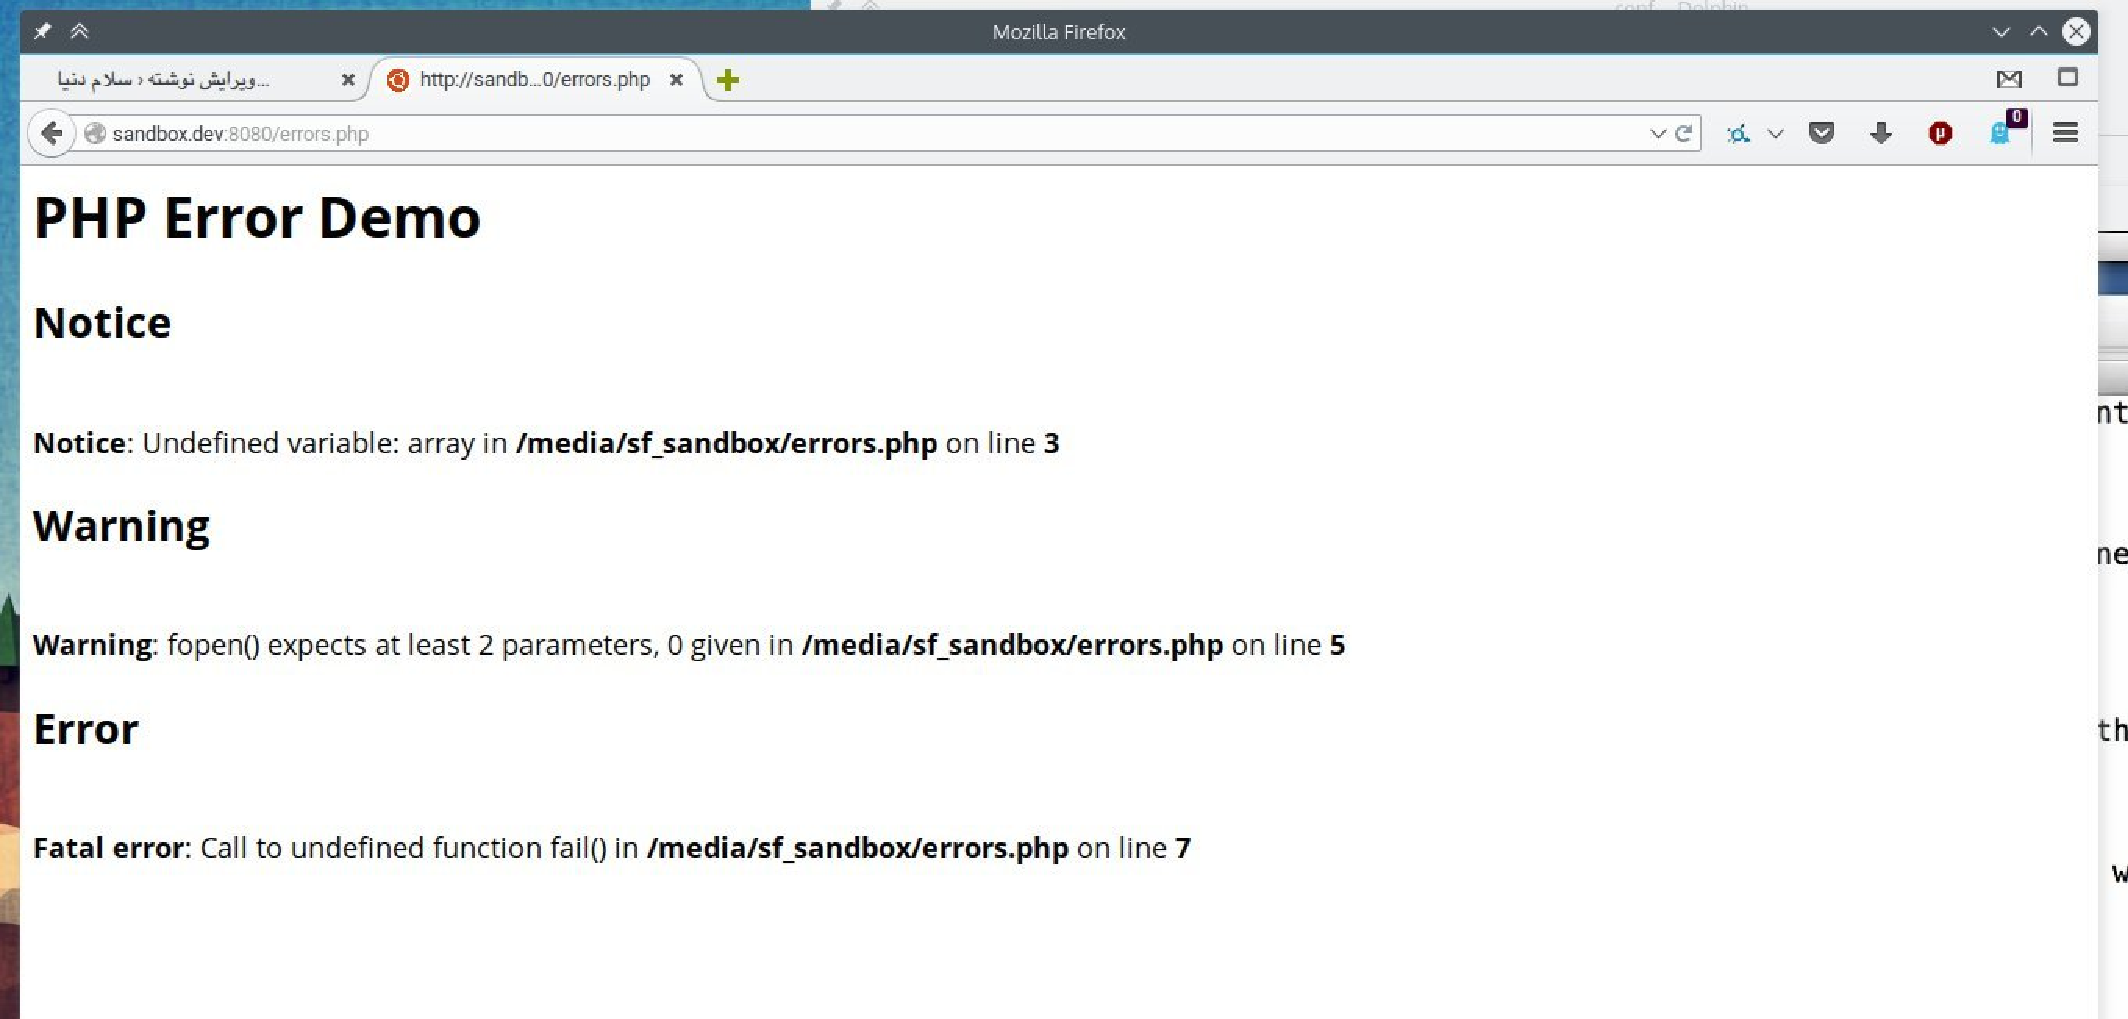
\includegraphics[width=.9\textwidth ,height=.45\textwidth]{Pic/PHP2}
    \caption{ نمایی از خطاهایی که در PHP رخ می دهند}
    \label{UbuntuServer-PHP-Error}
\end{figure}

همانطور که در تصویر نیز مشخص است؛ تمامی خطاها و هشدارهای رخ داده به کاربر نمایش داده خواهند شد. در این زمان با مطالعه پیغام هشدار و خطا به رفع آنان اقدام خواهید کرد. همچنین اگر به فایل لاگ ایجاد شده در این آموزش نیز مراجعه کنید؛ با خطاهای رخ داده در این فایل مواجه خواهید شد.
\newline
\begin{latin}  
    \lstinputlisting[numbers=right,language=Bash, framexleftmargin=5mm, frame=shadowbox,rulesepcolor=\color{Black}]{Code/codephp12.sh}
\end{latin}
    
 \section{ تنظیم و استفاده از مای‌اس‌کیوال}
 «مای‌اس‌کیوال (به انگلیسی: MySQL) یک سامانه مدیریت پایگاه داده‌ها متن‌باز است، که توسط شرکت اوراکل توسعه، توزیع، و پشتیبانی می‌شود.
 سرور مای‌اس‌کیوال به چندین کاربر اجازه استفاده همزمان از داده‌ها را می‌دهد.» 
 
\begin{flushleft}
     (ویکی‌پدیا ، دانشنامه آزاد)
\end{flushleft}
 
 در این بخش قصد داریم تا مای‌اس‌کیوال را تنظیم کنیم. تنظیمات مای‌اس‌کیوال نیز در شاخه «etc/» واقع شده‌است. تنظیمات اصلی مای‌اس‌کیوال در فایلی با نام «my.cnf» قرار دارد که با دستور زیر آن را ویرایش می‌کنیم.
 \newline
 \begin{latin}  
     \lstinputlisting[numbers=right,language=Bash, framexleftmargin=5mm, frame=shadowbox,rulesepcolor=\color{Black}]{Code/codephp13.sh}
    \end{latin}
    بعد از آنکه فایل بالا را باز کردید؛ قسمت‌های مشخص شده زیر ا در آن تغییر دهید. برای رفتن به بخش‌های مورد نیاز در این ویرایشگر متنی از کلید‌های 
    \path{«CTRL + W»}
     استفاده کنید و سپس عبارت مورد نظر برای جستجو در فایل را وارد کنید. بعد از وارد کردن عبارت مورد نظر؛ شما به خطی که آن عبارت یافت شده‌است خواهید رفت. برای اولین تغییر با استفاده از روش گفته شده؛ به دنبال عبارت «skip-external-locking» بگردید و با یافتن آن، خط جدیدی را زیر آن اضافه کرده و مقادیر زیر را برای پشتیبانی از واژه‌ها و حروف UTF-8 وارد کنید.
  \newline
  \begin{latin}  
      \lstinputlisting[numbers=right,language=Bash, framexleftmargin=5mm, frame=shadowbox,rulesepcolor=\color{Black}]{Code/mysql.conf.txt}
    \end{latin}
    تنظیمات مای‌اس‌کیوال به شکلی تنظیم شده است که فقط از طریق آدرس محلی 127.0.0.1 قادر به دسترسی به آن هستید. برای آنکه بتوانید با هر آدرس آی‌پی به آن دسترسی داشته باشید. با استفاده از روش مذکور عبارت «bind-address» را جستجو کرده و آدرس مقابل عبارت بالا را به مورد زیر تغییر دهید.
\newline
 \begin{latin}  
 \lstinputlisting[numbers=right,language=Bash, framexleftmargin=5mm, frame=shadowbox,rulesepcolor=\color{Black}]{Code/mysql.conf2.txt}
\end{latin}
همچنین برای فعال کردن قابلیت 
\path{«slow-quey-log»}
 نیز عبارت 
\path{«log_slow_queries»}
 را جست‌وجو کرده و با یافتن خطی که این عبارت در آن وجود دارد مقادیر زیر را در خط جدیدی در بالای عبارت یافت شده وارد کنید.
\newline
\begin{latin}  
    \lstinputlisting[numbers=right,language=SH, framexleftmargin=5mm, frame=shadowbox,rulesepcolor=\color{Black}]{Code/mysql.conf3.txt}
\end{latin}
برای تغییر کلید بافر نیز عبارت 
\path{«key_buffer»}
 را در فایل جست‌وجو کرده و در خط یافت شده؛ عبارت بالا را به عبارت 
\path{«key_buffer_size»}
  تغییر دهید.
\newline
\begin{latin}  
    \lstinputlisting[numbers=right,language=SH, framexleftmargin=5mm, frame=shadowbox,rulesepcolor=\color{Black}]{Code/mysql.conf4.txt}
\end{latin}
با جستجوی مجدد عبارت 
\path{«key_buffer» }
عبارت دیگر را نیز به عبارت جدید 
\path{«key_buffer_size»}
 تغییر دهید.
 \newline
 \begin{latin}  
     \lstinputlisting[numbers=right,language=SH, framexleftmargin=5mm, frame=shadowbox,rulesepcolor=\color{Black}]{Code/mysql.conf5.txt}
 \end{latin}
 بعد از انجام تغییرات بالا، فایل تنظیمات را با کلید‌های میانبر «CTRL + X» و نوشتن واژه وای «Y» ذخیره کنید. برای استفاده از تنظیمات جدید سرویس مای‌اس‌کیوال را راه‌اندازی مجدد کنید. برای راه‌اندازی مجدد این سرویس از دستور زیر استفاده می‌شود. (گفتنی است در نسخه‌های جدید که از SystemD استفاده می‌شود باید از دستور دیگری استفاده کنید؛ با این حال دستور زیر برای ویرایش‌های جدید، قادر است دستور مشابه در  نسخه‌های جدید اوبونتو و بهره‌مند از سیستم‌دی را اجرا کند. )
 \newline
 \begin{latin}  
     \lstinputlisting[numbers=right,language=SH, framexleftmargin=5mm, frame=shadowbox,rulesepcolor=\color{Black}]{Code/mysql.conf6.txt}
    \end{latin}
بعد از اینکه سرویس بالا مجددا راه‌اندازی شد؛ باید دسترسی‌ها برای کاربر ریشه را در جدول دسترسی‌ها اضافه و دسترسی‌ها را به‌روز کنید. در این زمان شما اختیارت کاربر ریشه را در دسترسی به جداول، کاربران و … فراهم خواهید کرد. برای این‌کار باید وارد ابزار مای‌اس‌کیوال شوید و برای اینکار دستورات زیر را اجرا کنید.
\newline
\begin{latin}  
    \lstinputlisting[numbers=right,language=SH, framexleftmargin=5mm, frame=shadowbox,rulesepcolor=\color{Black}]{Code/mysql.conf7.txt}
\end{latin}
بعد از مشاهده اعلان مای‌اس‌کیوال دستور زیر را در آن وارد کنید تا مجوزهای کاربر ریشه، به‌روز شود.
\newline
\begin{latin}  
    \lstinputlisting[numbers=right,language=SH, framexleftmargin=5mm, frame=shadowbox,rulesepcolor=\color{Black}]{Code/mysql.conf8.txt}
\end{latin}

سپس دستور زیر را نیز اجرا نمایید تا مجوزها و دسترسی‌ها یک‌بار دیگر از نو تخصیص یابد.
\newline
\begin{latin}  
    \lstinputlisting[numbers=right,language=SH, framexleftmargin=5mm, frame=shadowbox,rulesepcolor=\color{Black}]{Code/mysql.conf9.txt}
\end{latin}
حال دیگر تنظیم مای‌اس‌کیوال به پایان رسیده است و می‌توانید با ابزار مورد نظر خود به آن متصل شوید. برای مدیریت و ساخت بانک‌های اطلاعاتی هم می‌توان از ابزار خود مای‌اس‌کیوال استفاده کرد و هم می‌توان از ابزارهای شخص ثالثی مانند پی‌اچ‌پی مای‌ادمین بهره جست.